\def\baselinestretch{1}
\section{Descrizione algoritmo}
\def\baselinestretch{1.66}
\thispagestyle{headings}

\subsection{Pseudo codice}\label{gg}
\indent Per calcolare i cammini minimi\footnote{Anche definiti
come albero dei cammini minimi radicati in una sorgente.} da una sorgente si \`e
scelto di utilizzare l'algoritmo greedy proposto dall'olandese \textbf{Edsger 
Dijkstra} che va a scegliere localmente 
un nodo adiacente pi\`u vicino a quello analizzato. Per
definizione della sottostruttura ottima di un cammino minimo, il
\textbf{primo wormhole} aggiunto nell'albero dei cammini minimi, \`e
quello che si pu\`o raggiungere pi\`u velocemente da una data
sorgente. Per tanto \`e stato modificato Dijkstra per salvare i womrhole che
incontra durante la creazione del cammino, e per fermarsi una volta raggiunta la destinazione.\newline
\indent L'algoritmo che verr\`a mostrato di seguito \`e il cuore
del programma: in input riceve i nodi sorgente e destinazione
e in fase di elaborazione restituisce \textbf{i cammini minimi}
dal nodo sorgente a quello destinazione. \`E stato usato
il plurale in quanto, potrebbe esserci un secondo cammino
che fa uso dei wormhole, o viceversa se il grafo non
\`e connesso, esserci solamente il cammino con i wormhole.\newline
\indent La procedura \textbf{Galactic Dijkstra} applica una prima volta 
Dijkstra dalla sorgente fino a che non trova la
destinazione e nel mentre salva tutti i wormhole che incontra,
estraendone solo il primo (riga 1).
Se esiste un wormhole nell'albero dei cammini minimi radicato in S,
allora si procede ad una seconda applicazione di Dijkstra, usando
come sorgente il nodo di destinazione. Se questi due wormhole
sono diversi allora si calcola il percorso minimo tra i due e si
aggiunge un arco simbolico di peso 1.\newline


\IncMargin{1.5em}
\begin{algorithm}[H]
\setstretch{1.1}
\caption{Galactic Dijkstra}
\SetKwData{Left}{left}\SetKwData{This}{this}\SetKwData{Up}{up}
\SetKwFunction{Union}{Union}\SetKwFunction{FindCompress}{FindCompress}
\SetKwInOut{Input}{input}\SetKwInOut{Result}{result}
\SetKwIF{If}{ElseIf}{Else}{if}{:}{elif}{else:}{}
\BlankLine\BlankLine
\Input{Source node $\in V$, Destination node $\in V$}
\Result{print fast path from $s$ to $d$, w/ {\bf and} w/o wormholes if any}
\BlankLine
\emph{$w_1$ = apply Dijkstra from $S$ and save first wormhole encountered}\;
$distance = printPath(s, d)$\;
\If{$\exists \ w_1$}{
    \emph{$w_2$ = apply Dijkstra from $D$ and save first wormhole encountered}\;
    \If{$\exists \ w2 \ {\bf and} \ w1 \neq w2$}{
        $dw_1$ = $printPath(s, w_1)$\;
        $dw_2$ = $printPath(w_2, d)$\;
        $d_{dw_1+dw_2}$ = $dw_1 + 1 + dw_2$\;
    }
}
\BlankLine
\end{algorithm}
\DecMargin{1em}

\subsection{Diagrammi delle classe e dettagli architetturali}
\subsubsection{Priority Queue e Heap}
\indent La coda di priorit\`a \`e stata sviluppata come detto in precedenza facendo uso
di un \textbf{Heap Binario}, per la precisione un Min Heap. Si poteva creare una classe generica 
priority queue e usare un \textbf{pattern comportamentale} (e.g. Strategy) per sfruttare la possibilit\`a
di cambiare comportamento (minima priorit\`a o massima) in base ad un flag in fase di creazione della classe.
Non \`e stato usato tale approccio in quanto nell'algoritmo di Dijkstra si fa uso solamente di una
coda a minima priotit\`a.\newline\indent Un' altra nota riguarda l'uso della classe Min Heap all'interno della
Priority Queue: sarebbe stato utile usare un' \textbf{interfaccia} (i.g. classe astratta) per l'heap dando
la possibilit\`a al programmatore di usare un altra tipologia (e.g.: Fibonacci, Brodal, Binomiale, etc.).
Non avendo usato tale approccio la classe Min Priority Queue \`e dipendente dall' Heap Binario.
\begin{center}
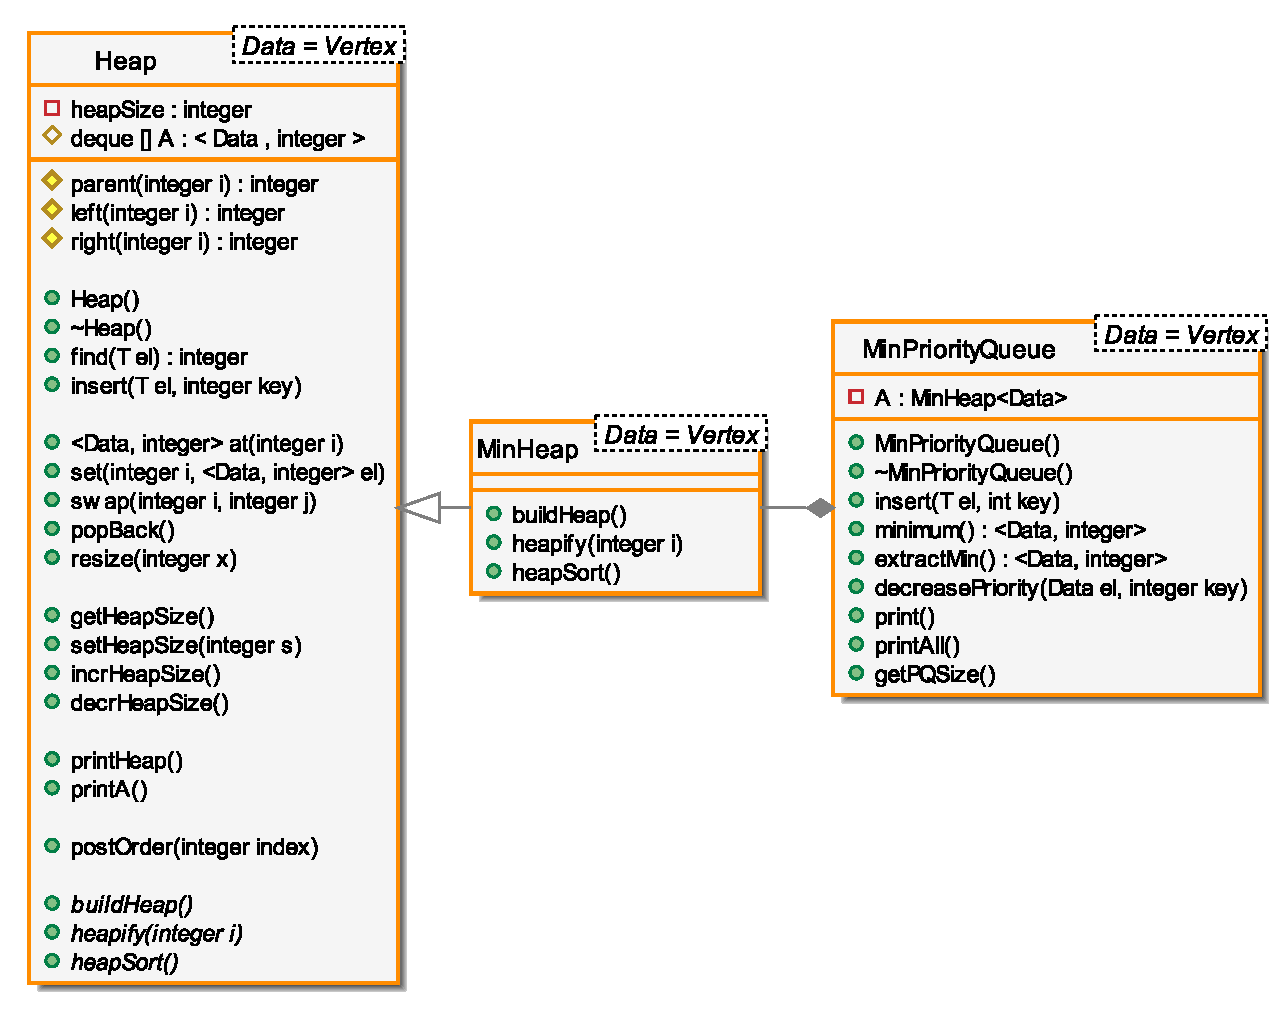
\includegraphics[scale=0.7]{tesina_tex/spacegraph/2img/pq.eps}
\captionof{figure}{Min priority Queue}
\end{center}
N.d.r.: ogni classe ha un parametro template Data, in questo caso specifico viene usato un puntatore ad
oggetto Vertex, mostrato di seguito.

\newpage
\subsubsection{Grafo e Vertici}
\indent Ogni elemento del grafo, i \textbf{Vertici}, sono dei nodi che ereditano da un generico "oggetto"
\textbf{Item} la possibilit\`a di inserire Dati indentificati da una chiave. A tal proposito non avendo
bisogno di conservare nessun dato si \`e deciso di usare come parametro del template un \textbf{puntatore
a void}. Ogni vertice ha una mappatura con i vertici \textbf{adiacenti} (realizzata tramite un hashtable
di tipo unordered), un riferimento al padre nell' albero dei cammini minimi, e la distanza dal nodo radice.
\newline\indent Il grafo possiede un vettore di puntatori a vertici e ha metodi per creare un albero
dei cammini minimi (Dijkstra), restituire o stampare il percorso da una sorgente e una destinazione.
Il metodo dijkstra \`e stato ridefinito in modo tale da poter eseguire operazioni aggiuntive alla fine
del rilassamento di un nodo estratto dalla coda: si pu\`o decidere di usare una funzione lambda oppure un
puntatore a funzione per inserire un \textbf{criterio di stop} nell'algoritmo (e.g. raggiunto un nodo
specifico), inoltre verr\`a restituito l'ultimo elemento estratto.\newline N.d.r.: il metodo dijkstra
internamente fa uso delle subroutine \textit{initSingleSource} e \textit{relax} come da
manuale\footnote{Vedere riferimenti bibliografici.} ma poich\`e tale implementazione
pu\`o cambiare (non far uso della Min Priority Queue ad esempio) si \`e deciso di non inserirle come
metodi privati durante la definizione della classe. Per cui verranno citate e mostrate solo per far capire
la connessione con la min priority queue.
\begin{center}
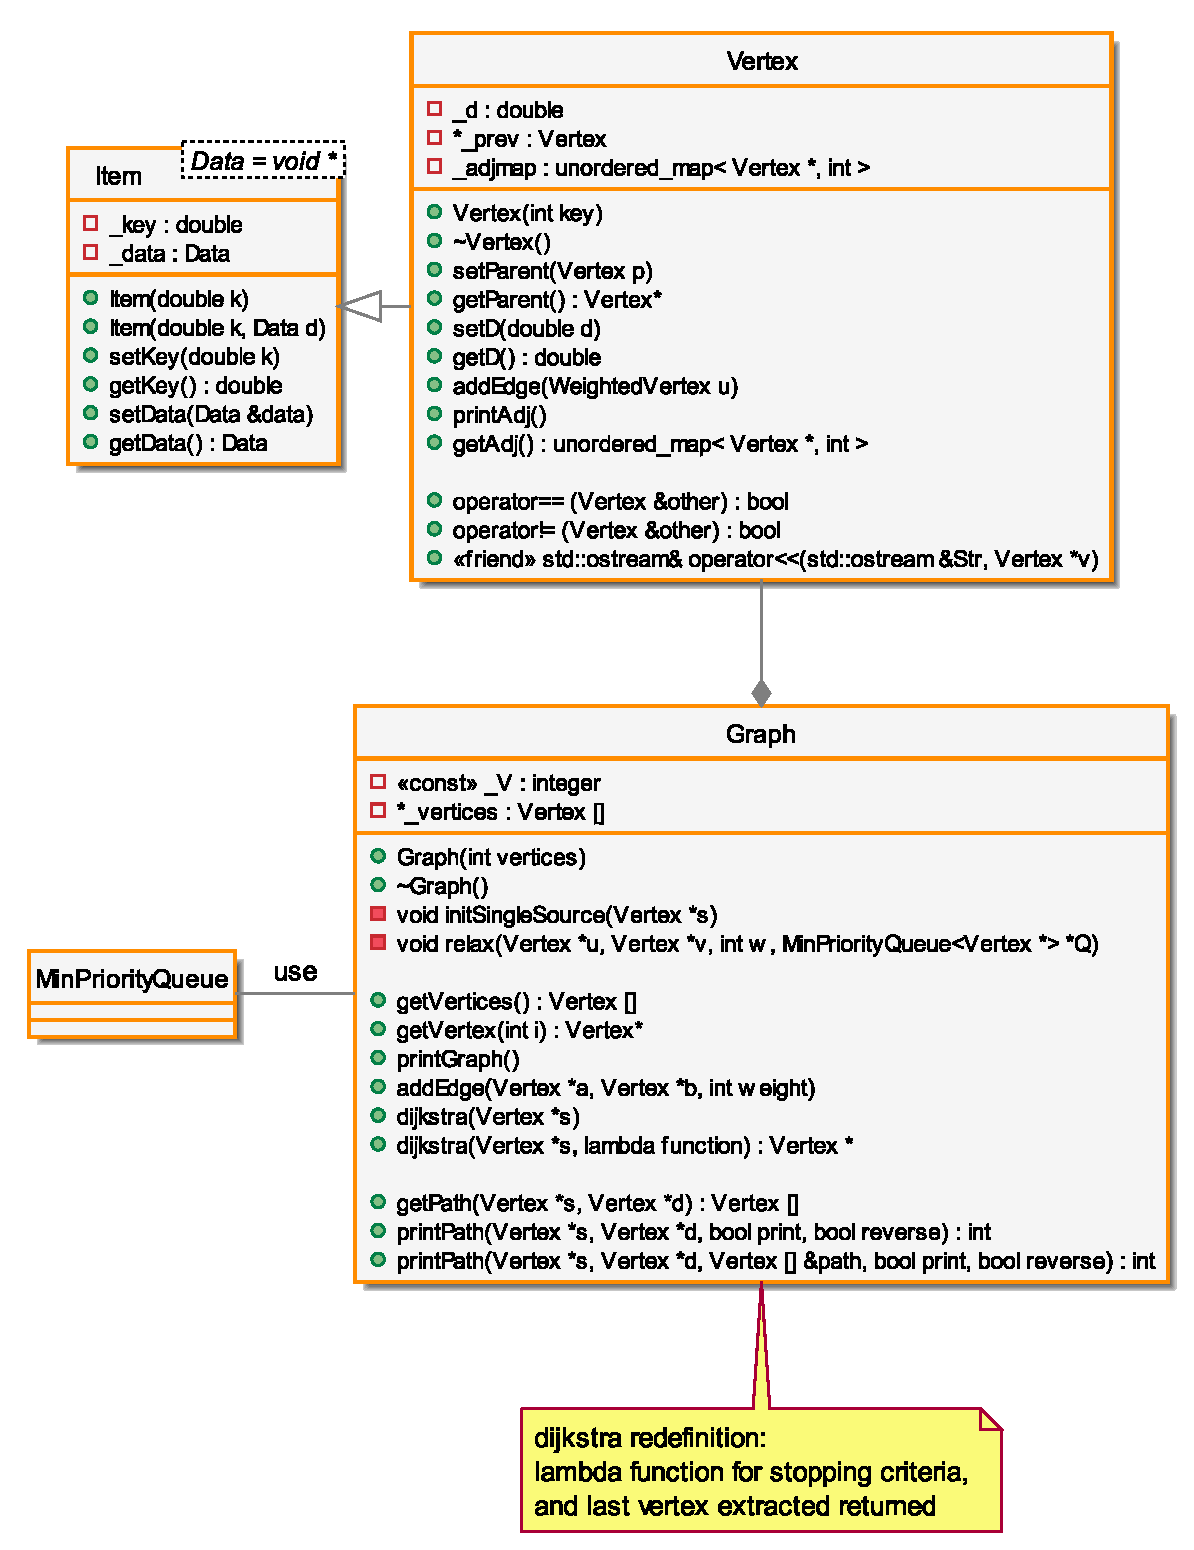
\includegraphics[scale=0.7]{tesina_tex/spacegraph/2img/g.eps}
\captionof{figure}{Vertici e Grafo}
\end{center}

\newpage
\subsubsection{Parser e Grafo galattico}
\indent Il main del programma usera la classe Parser per creare e instanziare correttamente un oggetto di
tipo GalacticGraph. Tale classe altro non \`e che una specializzazione del grafo base, con l'aggiunta
di una mappatura dei wormhole del sistema caricato e dell' algortimo Galactic Dijkstra (par. \ref{gg}).
\begin{center}
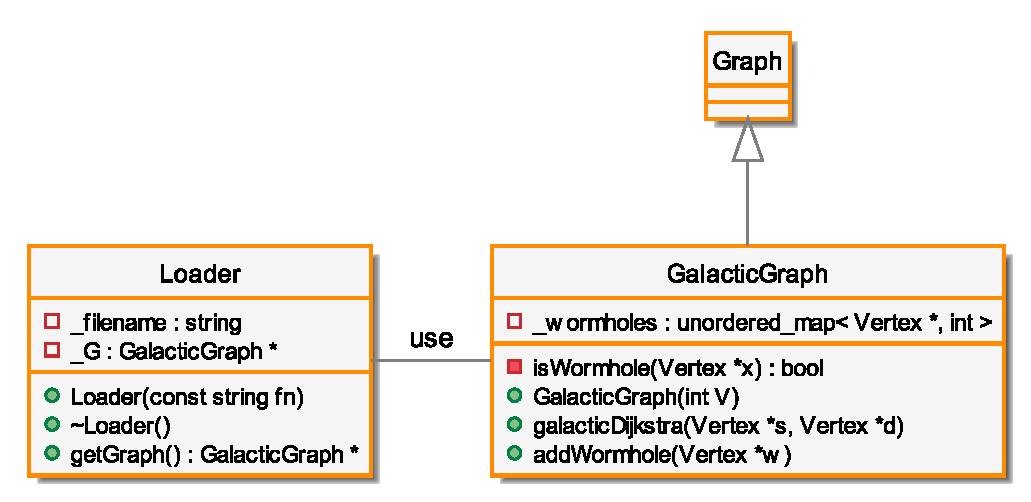
\includegraphics[scale=0.9]{tesina_tex/spacegraph/2img/gg.eps}
\captionof{figure}{Loader e Grago galattico}
\end{center}